\chapter{Lý thuyết số}

\index{number theory}

\key{Lý thuyết số (Number theory)} là một nhánh của toán học
nghiên cứu về các số nguyên.
Lý thuyết số là một lĩnh vực hấp dẫn,
bởi vì nhiều câu hỏi liên quan đến số nguyên
rất khó giải quyết mặc dù chúng
trông có vẻ đơn giản thoạt nhìn.

Ví dụ, hãy xem xét phương trình sau:
\[x^3 + y^3 + z^3 = 33\]
Dễ dàng tìm thấy ba số thực $x$, $y$ và $z$
thỏa mãn phương trình.
Ví dụ, chúng ta có thể chọn
\[
\begin{array}{lcl}
x = 3, \\
y = \sqrt[3]{3}, \\
z = \sqrt[3]{3}.\\
\end{array}
\]
Tuy nhiên, đó là một bài toán mở trong lý thuyết số
liệu có ba
\emph{số nguyên} $x$, $y$ và $z$ nào
thỏa mãn phương trình hay không \cite{bec07}.

Trong chương này, chúng ta sẽ tập trung vào các khái niệm cơ bản
và các thuật toán trong lý thuyết số.
Trong suốt chương, chúng ta sẽ giả định rằng tất cả các số
đều là số nguyên, trừ khi có quy định khác.

\section{Số nguyên tố và ước số}

\index{divisibility}
\index{factor}
\index{divisor}

Một số $a$ được gọi là một \key{thừa số (factor)} hoặc một \key{ước số (divisor)} của một số $b$
nếu $a$ chia hết cho $b$.
Nếu $a$ là một thừa số của $b$,
chúng ta viết $a \mid b$, và ngược lại chúng ta viết $a \nmid b$.
Ví dụ, các ước số của 24 là
1, 2, 3, 4, 6, 8, 12 và 24.

\index{prime}
\index{prime decomposition}

Một số $n>1$ là một \key{số nguyên tố (prime)}
nếu các ước số dương duy nhất của nó là 1 và $n$.
Ví dụ, 7, 19 và 41 là các số nguyên tố,
nhưng 35 không phải là một số nguyên tố, vì $5 \cdot 7 = 35$.
Với mọi số $n>1$, có một
\key{phân tích ra thừa số nguyên tố (prime factorization)} duy nhất
\[ n = p_1^{\alpha_1} p_2^{\alpha_2} \cdots p_k^{\alpha_k},\]
trong đó $p_1,p_2,\ldots,p_k$ là các số nguyên tố phân biệt và
$\alpha_1,\alpha_2,\ldots,\alpha_k$ là các số dương.
Ví dụ, phân tích ra thừa số nguyên tố của 84 là
\[84 = 2^2 \cdot 3^1 \cdot 7^1.\]

\key{Số lượng các ước số} của một số $n$ là
\[\tau(n)=\prod_{i=1}^k (\alpha_i+1),\]
bởi vì với mỗi số nguyên tố $p_i$, có
$\alpha_i+1$ cách để chọn số lần
nó xuất hiện trong ước số.
Ví dụ, số lượng các ước số
của 84 là
$\tau(84)=3 \cdot 2 \cdot 2 = 12$.
Các ước số là
1, 2, 3, 4, 6, 7, 12, 14, 21, 28, 42 và 84.

\key{Tổng các ước số} của $n$ là
\[\sigma(n)=\prod_{i=1}^k (1+p_i+\ldots+p_i^{\alpha_i}) = \prod_{i=1}^k \frac{p_i^{a_i+1}-1}{p_i-1},\]
trong đó công thức sau dựa trên công thức cấp số nhân.
Ví dụ, tổng các ước số của 84 là
\[\sigma(84)=\frac{2^3-1}{2-1} \cdot \frac{3^2-1}{3-1} \cdot \frac{7^2-1}{7-1} = 7 \cdot 4 \cdot 8 = 224.\]

\key{Tích các ước số} của $n$ là
\[\mu(n)=n^{\tau(n)/2},\]
bởi vì chúng ta có thể tạo thành $\tau(n)/2$ cặp từ các ước số,
mỗi cặp có tích là $n$.
Ví dụ, các ước số của 84
tạo ra các cặp
$1 \cdot 84$, $2 \cdot 42$, $3 \cdot 28$, v.v.,
và tích của các ước số là $\mu(84)=84^6=351298031616$.

\index{perfect number}

Một số $n$ được gọi là một \key{số hoàn hảo (perfect number)} nếu $n=\sigma(n)-n$,
tức là, $n$ bằng tổng các ước số của nó
trong khoảng từ $1$ đến $n-1$.
Ví dụ, 28 là một số hoàn hảo,
bởi vì $28=1+2+4+7+14$.

\subsubsection{Số lượng các số nguyên tố}

Dễ dàng chứng minh rằng có vô số
số nguyên tố.
Nếu số lượng các số nguyên tố là hữu hạn,
chúng ta có thể xây dựng một tập hợp $P=\{p_1,p_2,\ldots,p_n\}$
chứa tất cả các số nguyên tố.
Ví dụ, $p_1=2$, $p_2=3$, $p_3=5$, và cứ thế.
Tuy nhiên, sử dụng $P$, chúng ta có thể tạo ra một số nguyên tố mới
\[p_1 p_2 \cdots p_n+1\]
lớn hơn tất cả các phần tử trong $P$.
Đây là một mâu thuẫn, và số lượng các số nguyên tố
phải là vô hạn.

\subsubsection{Mật độ của các số nguyên tố}

Mật độ của các số nguyên tố có nghĩa là các số nguyên tố xuất hiện
thường xuyên như thế nào trong các số.
Gọi $\pi(n)$ là số lượng các số nguyên tố trong khoảng từ
$1$ đến $n$. Ví dụ, $\pi(10)=4$, bởi vì
có 4 số nguyên tố trong khoảng từ $1$ đến $10$: 2, 3, 5 và 7.

Có thể chứng minh rằng
\[\pi(n) \approx \frac{n}{\ln n},\]
điều này có nghĩa là các số nguyên tố khá thường xuyên.
Ví dụ, số lượng các số nguyên tố trong khoảng từ
$1$ đến $10^6$ là $\pi(10^6)=78498$,
và $10^6 / \ln 10^6 \approx 72382$.

\subsubsection{Các giả thuyết}

Có nhiều \emph{giả thuyết} liên quan đến các số nguyên tố.
Hầu hết mọi người nghĩ rằng các giả thuyết là đúng,
nhưng không ai có thể chứng minh chúng.
Ví dụ, các giả thuyết sau đây là nổi tiếng:

\begin{itemize}
\index{Goldbach's conjecture}
\item \key{Giả thuyết Goldbach (Goldbach's conjecture)}:
Mỗi số nguyên chẵn $n>2$ có thể được biểu diễn dưới dạng
tổng $n=a+b$ sao cho cả $a$ và $b$ đều là các số nguyên tố.
\index{twin prime}
\item \key{Giả thuyết số nguyên tố sinh đôi (Twin prime conjecture)}:
Có vô số cặp
có dạng $\{p,p+2\}$,
trong đó cả $p$ và $p+2$ đều là các số nguyên tố.
\index{Legendre's conjecture}
\item \key{Giả thuyết Legendre (Legendre's conjecture)}:
Luôn có một số nguyên tố giữa các số
$n^2$ và $(n+1)^2$, trong đó $n$ là một số nguyên dương bất kỳ.
\end{itemize}

\subsubsection{Các thuật toán cơ bản}

Nếu một số $n$ không phải là số nguyên tố,
nó có thể được biểu diễn dưới dạng một tích $a \cdot b$,
trong đó $a \le \sqrt n$ hoặc $b \le \sqrt n$,
vì vậy nó chắc chắn có một ước số trong khoảng từ $2$ đến $\lfloor \sqrt n \rfloor$.
Sử dụng quan sát này, chúng ta có thể vừa kiểm tra
xem một số có phải là số nguyên tố hay không vừa tìm phân tích ra thừa số nguyên tố
của một số trong thời gian $O(\sqrt n)$.

Hàm \texttt{prime} sau đây kiểm tra
xem số đã cho $n$ có phải là số nguyên tố hay không.
Hàm cố gắng chia $n$ cho
tất cả các số trong khoảng từ $2$ đến $\lfloor \sqrt n \rfloor$,
và nếu không có số nào trong số đó chia hết cho $n$, thì $n$ là số nguyên tố.

\begin{lstlisting}
bool prime(int n) {
    if (n < 2) return false;
    for (int x = 2; x*x <= n; x++) {
        if (n%x == 0) return false;
    }
    return true;
}
\end{lstlisting}

\noindent
Hàm \texttt{factors} sau đây
xây dựng một vector chứa phân tích ra thừa số
nguyên tố của $n$.
Hàm chia $n$ cho các thừa số nguyên tố của nó,
và thêm chúng vào vector.
Quá trình kết thúc khi số $n$ còn lại
không có ước số nào trong khoảng từ $2$ đến $\lfloor \sqrt n \rfloor$.
Nếu $n>1$, nó là số nguyên tố và là thừa số cuối cùng.

\begin{lstlisting}
vector<int> factors(int n) {
    vector<int> f;
    for (int x = 2; x*x <= n; x++) {
        while (n%x == 0) {
            f.push_back(x);
            n /= x;
        }
    }
    if (n > 1) f.push_back(n);
    return f;
}
\end{lstlisting}

Lưu ý rằng mỗi thừa số nguyên tố xuất hiện trong vector
nhiều lần bằng số lần nó chia hết cho số đó.
Ví dụ, $24=2^3 \cdot 3$,
vì vậy kết quả của hàm là $[2,2,2,3]$.

\subsubsection{Sàng Eratosthenes}

\index{sieve of Eratosthenes}

\key{Sàng Eratosthenes (sieve of Eratosthenes)}
là một thuật toán tiền xử lý
xây dựng một mảng mà chúng ta có thể
sử dụng để kiểm tra hiệu quả xem một số đã cho trong khoảng từ $2 \ldots n$
có phải là số nguyên tố hay không và, nếu không, tìm một thừa số nguyên tố của số đó.

Thuật toán xây dựng một mảng $\texttt{sieve}$
mà các vị trí $2,3,\ldots,n$ được sử dụng.
Giá trị $\texttt{sieve}[k]=0$ có nghĩa là
$k$ là số nguyên tố,
và giá trị $\texttt{sieve}[k] \neq 0$
có nghĩa là $k$ không phải là số nguyên tố và một
trong các thừa số nguyên tố của nó là $\texttt{sieve}[k]$.

Thuật toán lặp qua các số
$2 \ldots n$ một cách lần lượt.
Mỗi khi một số nguyên tố mới $x$ được tìm thấy,
thuật toán ghi lại rằng các bội số
của $x$ ($2x,3x,4x,\ldots$) không phải là số nguyên tố,
bởi vì số $x$ chia hết cho chúng.

Ví dụ, nếu $n=20$, mảng như sau:

\begin{center}
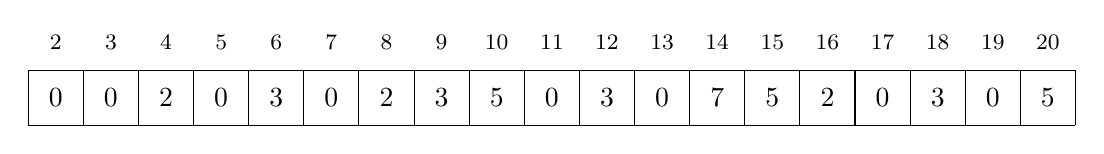
\begin{tikzpicture}[scale=0.7]
\draw (0,0) grid (19,1);

\node at (0.5,0.5) {$0$};
\node at (1.5,0.5) {$0$};
\node at (2.5,0.5) {$2$};
\node at (3.5,0.5) {$0$};
\node at (4.5,0.5) {$3$};
\node at (5.5,0.5) {$0$};
\node at (6.5,0.5) {$2$};
\node at (7.5,0.5) {$3$};
\node at (8.5,0.5) {$5$};
\node at (9.5,0.5) {$0$};
\node at (10.5,0.5) {$3$};
\node at (11.5,0.5) {$0$};
\node at (12.5,0.5) {$7$};
\node at (13.5,0.5) {$5$};
\node at (14.5,0.5) {$2$};
\node at (15.5,0.5) {$0$};
\node at (16.5,0.5) {$3$};
\node at (17.5,0.5) {$0$};
\node at (18.5,0.5) {$5$};

\footnotesize

\node at (0.5,1.5) {$2$};
\node at (1.5,1.5) {$3$};
\node at (2.5,1.5) {$4$};
\node at (3.5,1.5) {$5$};
\node at (4.5,1.5) {$6$};
\node at (5.5,1.5) {$7$};
\node at (6.5,1.5) {$8$};
\node at (7.5,1.5) {$9$};
\node at (8.5,1.5) {$10$};
\node at (9.5,1.5) {$11$};
\node at (10.5,1.5) {$12$};
\node at (11.5,1.5) {$13$};
\node at (12.5,1.5) {$14$};
\node at (13.5,1.5) {$15$};
\node at (14.5,1.5) {$16$};
\node at (15.5,1.5) {$17$};
\node at (16.5,1.5) {$18$};
\node at (17.5,1.5) {$19$};
\node at (18.5,1.5) {$20$};

\end{tikzpicture}
\end{center}

Đoạn mã sau đây triển khai sàng
Eratosthenes.
Đoạn mã giả định rằng mỗi phần tử của
\texttt{sieve} ban đầu bằng không.

\begin{lstlisting}
for (int x = 2; x <= n; x++) {
    if (sieve[x]) continue;
    for (int u = 2*x; u <= n; u += x) {
        sieve[u] = x;
    }
}
\end{lstlisting}

Vòng lặp bên trong của thuật toán được thực hiện
$n/x$ lần cho mỗi giá trị của $x$.
Do đó, một giới hạn trên cho thời gian chạy
của thuật toán là tổng điều hòa
\[\sum_{x=2}^n n/x = n/2 + n/3 + n/4 + \cdots + n/n = O(n \log n).\]

\index{harmonic sum}

Thực tế, thuật toán hiệu quả hơn,
bởi vì vòng lặp bên trong sẽ chỉ được thực hiện nếu
số $x$ là số nguyên tố.
Có thể chứng minh rằng thời gian chạy của
thuật toán chỉ là $O(n \log \log n)$,
một độ phức tạp rất gần với $O(n)$. 

\subsubsection{Thuật toán Euclid}

\index{greatest common divisor}
\index{least common multiple}
\index{Euclid's algorithm}

\key{Ước chung lớn nhất (greatest common divisor)} của
các số $a$ và $b$, $\gcd(a,b)$,
là số lớn nhất chia hết cho cả $a$ và $b$,
và \key{bội chung nhỏ nhất (least common multiple)} của
$a$ và $b$, $\textrm{lcm}(a,b)$,
là số nhỏ nhất chia hết cho
cả $a$ và $b$.
Ví dụ,
$\gcd(24,36)=12$ và
$\textrm{lcm}(24,36)=72$.

Ước chung lớn nhất và bội chung nhỏ nhất
có mối liên hệ như sau:
\[\textrm{lcm}(a,b)=\frac{ab}{\textrm{gcd}(a,b)}\]

\key{Thuật toán Euclid (Euclid's algorithm)}\footnote{Euclid là một nhà toán học người Hy Lạp sống vào khoảng năm 300 TCN. Đây có lẽ là thuật toán đầu tiên được biết đến trong lịch sử.} cung cấp một cách hiệu quả
để tìm ước chung lớn nhất của hai số.
Thuật toán dựa trên công thức sau:
\begin{equation*}
    \textrm{gcd}(a,b) = \begin{cases}
               a        & b = 0\\
               \textrm{gcd}(b,a \bmod b) & b \neq 0\\
           \end{cases}
\end{equation*}

Ví dụ,
\[\textrm{gcd}(24,36) = \textrm{gcd}(36,24)
= \textrm{gcd}(24,12) = \textrm{gcd}(12,0)=12.\]

Thuật toán có thể được triển khai như sau:
\begin{lstlisting}
int gcd(int a, int b) {
    if (b == 0) return a;
    return gcd(b, a%b);
}
\end{lstlisting}

Có thể chứng minh rằng thuật toán Euclid hoạt động
trong thời gian $O(\log n)$, trong đó $n=\min(a,b)$.
Trường hợp xấu nhất cho thuật toán là
trường hợp khi $a$ và $b$ là các số Fibonacci liên tiếp.
Ví dụ,
\[\textrm{gcd}(13,8)=\textrm{gcd}(8,5)
=\textrm{gcd}(5,3)=\textrm{gcd}(3,2)=\textrm{gcd}(2,1)=\textrm{gcd}(1,0)=1.\]

\subsubsection{Hàm phi Euler}

\index{coprime}
\index{Euler's totient function}

Các số $a$ và $b$ là \key{nguyên tố cùng nhau (coprime)}
nếu $\textrm{gcd}(a,b)=1$.
\key{Hàm phi Euler (Euler's totient function)} $\varphi(n)$
cho ra số lượng các số nguyên tố cùng nhau với $n$
trong khoảng từ $1$ đến $n$.
Ví dụ, $\varphi(12)=4$,
bởi vì 1, 5, 7 và 11
là nguyên tố cùng nhau với 12.

Giá trị của $\varphi(n)$ có thể được tính
từ phân tích ra thừa số nguyên tố của $n$
bằng công thức
\[ \varphi(n) = \prod_{i=1}^k p_i^{\alpha_i-1}(p_i-1). \]
Ví dụ, $\varphi(12)=2^1 \cdot (2-1) \cdot 3^0 \cdot (3-1)=4$.
Lưu ý rằng $\varphi(n)=n-1$ nếu $n$ là số nguyên tố.

\section{Số học mô-đun}

\index{modular arithmetic}

Trong \key{số học mô-đun (modular arithmetic)},
tập hợp các số bị giới hạn sao cho
chỉ có các số $0,1,2,\ldots,m-1$ được sử dụng,
trong đó $m$ là một hằng số.
Mỗi số $x$ được
biểu diễn bằng số $x \bmod m$:
phần dư sau khi chia $x$ cho $m$.
Ví dụ, nếu $m=17$, thì $75$
được biểu diễn bằng $75 \bmod 17 = 7$.

Thường thì chúng ta có thể lấy phần dư trước khi thực hiện
các phép tính.
Cụ thể, các công thức sau đây đúng:
\[
\begin{array}{rcl}
(x+y) \bmod m & = & (x \bmod m + y \bmod m) \bmod m \\
(x-y) \bmod m & = & (x \bmod m - y \bmod m) \bmod m \\
(x \cdot y) \bmod m & = & (x \bmod m \cdot y \bmod m) \bmod m \\
x^n \bmod m & = & (x \bmod m)^n \bmod m \\
\end{array}
\]

\subsubsection{Lũy thừa mô-đun}

Thường có nhu cầu tính toán hiệu quả
giá trị của $x^n \bmod m$.
Điều này có thể được thực hiện trong thời gian $O(\log n)$
sử dụng công thức đệ quy sau:
\begin{equation*}
    x^n = \begin{cases}
               1        & n = 0\\
               x^{n/2} \cdot x^{n/2} & \text{$n$ là số chẵn}\\
               x^{n-1} \cdot x & \text{$n$ là số lẻ}
           \end{cases}
\end{equation*}

Điều quan trọng là trong trường hợp $n$ chẵn,
giá trị của $x^{n/2}$ chỉ được tính một lần.
Điều này đảm bảo rằng độ phức tạp thời gian của
thuật toán là $O(\log n)$, bởi vì $n$ luôn được chia đôi
khi nó chẵn.

Hàm sau tính giá trị của
$x^n \bmod m$:

\begin{lstlisting}
int modpow(int x, int n, int m) {
    if (n == 0) return 1%m;
    long long u = modpow(x,n/2,m);
    u = (u*u)%m;
    if (n%2 == 1) u = (u*x)%m;
    return u;
}
\end{lstlisting}

\subsubsection{Định lý Fermat và Định lý Euler}

\index{Fermat's theorem}
\index{Euler's theorem}

\key{Định lý Fermat (Fermat's theorem)}
phát biểu rằng
\[x^{m-1} \bmod m = 1\]
khi $m$ là số nguyên tố và $x$ và $m$ là nguyên tố cùng nhau.
Điều này cũng cho ra
\[x^k \bmod m = x^{k \bmod (m-1)} \bmod m.\]
Tổng quát hơn, \key{Định lý Euler (Euler's theorem)}
phát biểu rằng
\[x^{\varphi(m)} \bmod m = 1\]
khi $x$ và $m$ là nguyên tố cùng nhau.
Định lý Fermat là một hệ quả của định lý Euler,
bởi vì nếu $m$ là một số nguyên tố, thì $\varphi(m)=m-1$.

\subsubsection{Nghịch đảo mô-đun}

\index{modular inverse}

Nghịch đảo của $x$ theo mô-đun $m$
là một số $x^{-1}$ sao cho
\[ x x^{-1} \bmod m = 1. \]
Ví dụ, nếu $x=6$ và $m=17$,
thì $x^{-1}=3$, bởi vì $6\cdot3 \bmod 17=1$.

Sử dụng nghịch đảo mô-đun, chúng ta có thể chia các số
theo mô-đun $m$, bởi vì phép chia cho $x$
tương ứng với phép nhân với $x^{-1}$.
Ví dụ, để đánh giá giá trị của $36/6 \bmod 17$,
chúng ta có thể sử dụng công thức $2 \cdot 3 \bmod 17$,
bởi vì $36 \bmod 17 = 2$ và $6^{-1} \bmod 17 = 3$.

Tuy nhiên, một nghịch đảo mô-đun không phải lúc nào cũng tồn tại.
Ví dụ, nếu $x=2$ và $m=4$, phương trình
\[ x x^{-1} \bmod m = 1 \]
không thể giải được, bởi vì tất cả các bội số của 2
đều chẵn và phần dư không bao giờ có thể là 1 khi $m=4$.
Hóa ra giá trị của $x^{-1} \bmod m$
có thể được tính chính xác khi $x$ và $m$ là nguyên tố cùng nhau.

Nếu một nghịch đảo mô-đun tồn tại, nó có thể được
tính bằng công thức
\[
x^{-1} = x^{\varphi(m)-1}.
\]
Nếu $m$ là số nguyên tố, công thức trở thành
\[
x^{-1} = x^{m-2}.
\]
Ví dụ,
\[6^{-1} \bmod 17 =6^{17-2} \bmod 17 = 3.\]

Công thức này cho phép chúng ta tính toán hiệu quả
các nghịch đảo mô-đun bằng thuật toán lũy thừa mô-đun.
Công thức có thể được suy ra bằng cách sử dụng định lý Euler.
Đầu tiên, nghịch đảo mô-đun phải thỏa mãn phương trình sau:
\[
x x^{-1} \bmod m = 1.
\]
Mặt khác, theo định lý Euler,
\[
x^{\varphi(m)} \bmod m =  xx^{\varphi(m)-1} \bmod m = 1,
\]
vì vậy các số $x^{-1}$ và $x^{\varphi(m)-1}$ bằng nhau.

\subsubsection{Số học máy tính}

Trong lập trình, các số nguyên không dấu được biểu diễn theo mô-đun $2^k$,
trong đó $k$ là số bit của kiểu dữ liệu.
Một hệ quả thông thường của điều này là một số sẽ quay vòng
nếu nó trở nên quá lớn.

Ví dụ, trong C++, các số thuộc kiểu \texttt{unsigned int}
được biểu diễn theo mô-đun $2^{32}$.
Đoạn mã sau khai báo một biến \texttt{unsigned int}
có giá trị là $123456789$.
Sau đó, giá trị này sẽ được nhân với chính nó,
và kết quả là
$123456789^2 \bmod 2^{32} = 2537071545$.

\begin{lstlisting}
unsigned int x = 123456789;
cout << x*x << "\n"; // 2537071545
\end{lstlisting}

\section{Giải phương trình}

\subsubsection*{Phương trình Diophantine}

\index{Diophantine equation}

Một \key{phương trình Diophantine (Diophantine equation)}
là một phương trình có dạng
\[ ax + by = c, \]
trong đó $a$, $b$ và $c$ là các hằng số
và các giá trị của $x$ và $y$ cần được tìm.
Mỗi số trong phương trình phải là một số nguyên.
Ví dụ, một nghiệm của phương trình
$5x+2y=11$ là $x=3$ và $y=-2$.

\index{extended Euclid's algorithm}

Chúng ta có thể giải quyết hiệu quả một phương trình Diophantine
bằng cách sử dụng thuật toán Euclid.
Hóa ra chúng ta có thể mở rộng thuật toán Euclid
để nó sẽ tìm ra các số $x$ và $y$
thỏa mãn phương trình sau:
\[
ax + by = \textrm{gcd}(a,b)
\]

Một phương trình Diophantine có thể được giải nếu
$c$ chia hết cho
$\textrm{gcd}(a,b)$,
và ngược lại nó không thể được giải.

Ví dụ, chúng ta hãy tìm các số $x$ và $y$
thỏa mãn phương trình sau:
\[
39x + 15y = 12
\]
Phương trình có thể được giải, bởi vì
$\textrm{gcd}(39,15)=3$ và $3 \mid 12$.
Khi thuật toán Euclid tính
ước chung lớn nhất của 39 và 15,
nó tạo ra chuỗi các lần gọi hàm sau:
\[
\textrm{gcd}(39,15) = \textrm{gcd}(15,9)
= \textrm{gcd}(9,6) = \textrm{gcd}(6,3)
= \textrm{gcd}(3,0) = 3 \]
Điều này tương ứng với các phương trình sau:
\[
\begin{array}{lcl}
39 - 2 \cdot 15 & = & 9 \\
15 - 1 \cdot 9 & = & 6 \\
9 - 1 \cdot 6 & = & 3 \\
\end{array}
\]
Sử dụng các phương trình này, chúng ta có thể suy ra
\[
39 \cdot 2 + 15 \cdot (-5) = 3
\]
và bằng cách nhân điều này với 4, kết quả là
\[
39 \cdot 8 + 15 \cdot (-20) = 12,
\]
vì vậy một nghiệm của phương trình là
$x=8$ và $y=-20$.

Một nghiệm của một phương trình Diophantine không phải là duy nhất,
bởi vì chúng ta có thể tạo ra vô số nghiệm
nếu chúng ta biết một nghiệm.
Nếu một cặp $(x,y)$ là một nghiệm, thì tất cả các cặp
\[(x+\frac{kb}{\textrm{gcd}(a,b)},y-\frac{ka}{\textrm{gcd}(a,b)})\]
cũng là nghiệm, trong đó $k$ là một số nguyên bất kỳ.

\subsubsection{Định lý số dư Trung Hoa}

\index{Chinese remainder theorem}

\key{Định lý số dư Trung Hoa (Chinese remainder theorem)} giải quyết
một nhóm các phương trình có dạng
\[
\begin{array}{lcl}
x & = & a_1 \bmod m_1 \\
x & = & a_2 \bmod m_2 \\
\cdots \\
x & = & a_n \bmod m_n \\
\end{array}
\]
trong đó tất cả các cặp $m_1,m_2,\ldots,m_n$ là nguyên tố cùng nhau.

Gọi $x^{-1}_m$ là nghịch đảo của $x$ theo mô-đun $m$, và
\[ X_k = \frac{m_1 m_2 \cdots m_n}{m_k}.\]
Sử dụng ký hiệu này, một nghiệm của các phương trình là
\[x = a_1 X_1 {X_1}^{-1}_{m_1} + a_2 X_2 {X_2}^{-1}_{m_2} + \cdots + a_n X_n {X_n}^{-1}_{m_n}.\]
Trong nghiệm này, với mỗi $k=1,2,\ldots,n$,
\[a_k X_k {X_k}^{-1}_{m_k} \bmod m_k = a_k,\]
bởi vì
\[X_k {X_k}^{-1}_{m_k} \bmod m_k = 1.\]
Vì tất cả các số hạng khác trong tổng đều chia hết cho $m_k$,
chúng không ảnh hưởng đến phần dư,
và $x \bmod m_k = a_k$.

Ví dụ, một nghiệm cho
\[
\begin{array}{lcl}
x & = & 3 \bmod 5 \\
x & = & 4 \bmod 7 \\
x & = & 2 \bmod 3 \\
\end{array}
\]
là
\[ 3 \cdot 21 \cdot 1 + 4 \cdot 15 \cdot 1 + 2 \cdot 35 \cdot 2 = 263.\]

Một khi chúng ta đã tìm thấy một nghiệm $x$,
chúng ta có thể tạo ra vô số nghiệm khác,
bởi vì tất cả các số có dạng
\[x+m_1 m_2 \cdots m_n\]
đều là nghiệm.

\section{Các kết quả khác}

\subsubsection{Định lý Lagrange}

\index{Lagrange's theorem}

\key{Định lý Lagrange (Lagrange's theorem)}
phát biểu rằng mọi số nguyên dương
có thể được biểu diễn dưới dạng tổng của bốn số chính phương, tức là,
$a^2+b^2+c^2+d^2$.
Ví dụ, số 123 có thể được biểu diễn
dưới dạng tổng $8^2+5^2+5^2+3^2$.

\subsubsection{Định lý Zeckendorf}

\index{Zeckendorf's theorem}
\index{Fibonacci number}

\key{Định lý Zeckendorf (Zeckendorf's theorem)}
phát biểu rằng mọi
số nguyên dương có một biểu diễn duy nhất
dưới dạng một tổng các số Fibonacci sao cho
không có hai số nào bằng nhau hoặc là
các số Fibonacci liên tiếp.
Ví dụ, số 74 có thể được biểu diễn
dưới dạng tổng $55+13+5+1$.

\subsubsection{Bộ ba Pythagoras}

\index{Pythagorean triple}
\index{Euclid's formula}

Một \key{bộ ba Pythagoras (Pythagorean triple)} là một bộ ba $(a,b,c)$
thỏa mãn định lý Pythagoras
$a^2+b^2=c^2$, có nghĩa là có một tam giác vuông
với các cạnh có độ dài $a$, $b$ và $c$.
Ví dụ, $(3,4,5)$ là một bộ ba Pythagoras.

Nếu $(a,b,c)$ là một bộ ba Pythagoras,
tất cả các bộ ba có dạng $(ka,kb,kc)$
cũng là các bộ ba Pythagoras trong đó $k>1$.
Một bộ ba Pythagoras là \emph{nguyên thủy} nếu
$a$, $b$ và $c$ là nguyên tố cùng nhau,
và tất cả các bộ ba Pythagoras có thể được xây dựng
từ các bộ ba nguyên thủy bằng cách sử dụng một hệ số nhân $k$.

\key{Công thức Euclid (Euclid's formula)} có thể được sử dụng để tạo ra
tất cả các bộ ba Pythagoras nguyên thủy.
Mỗi bộ ba như vậy có dạng
\[(n^2-m^2,2nm,n^2+m^2),\]
trong đó $0<m<n$, $n$ và $m$ là nguyên tố cùng nhau
và ít nhất một trong $n$ và $m$ là số chẵn.
Ví dụ, khi $m=1$ và $n=2$, công thức
tạo ra bộ ba Pythagoras nhỏ nhất
\[(2^2-1^2,2\cdot2\cdot1,2^2+1^2)=(3,4,5).\]

\subsubsection{Định lý Wilson}

\index{Wilson's theorem}

\key{Định lý Wilson (Wilson's theorem)}
phát biểu rằng một số $n$
là số nguyên tố chính xác khi
\[(n-1)! \bmod n = n-1.\]
Ví dụ, số 11 là số nguyên tố, bởi vì
\[10! \bmod 11 = 10,\]
và số 12 không phải là số nguyên tố, bởi vì
\[11! \bmod 12 = 0 \neq 11.\]

Do đó, định lý Wilson có thể được sử dụng để tìm ra
xem một số có phải là số nguyên tố hay không. Tuy nhiên, trong thực tế, định lý không thể được
áp dụng cho các giá trị lớn của $n$, bởi vì rất khó
để tính các giá trị của $(n-1)!$ khi $n$ lớn.